\chapter{Discussion}\label{ch:Discussion}\addtocontents{lof}{\protect\contentsline{chapter}{\protect\numberline{\thechapter}Discussion}{}{}}
% \newthought{Synopsis}\synopsisMethod

\section{Challenges and Discussion of Methodology}

\newthought{Mould Die Design}
The challenges in the early stages of the study with imported anatomic valve geometries not allowing for feature interaction in SolidWorks prompted some very suboptimal design choices that were very time intensive to work around. The series of 2-stage epoxy moulds developed as discussed in \cref{fig:moulddie} had a 72 hour curing time, which made any design inputs learned much slower to implement.

This process became obselete when the software package was updated as it was discovered that the 'Segment Mesh' tool previously attempted to use to convert the STL mesh body to a solid part had been overall to allow more complex geometries to be segmented. On this discovery the part was successfully converted to a solid body which allowed it to be subtracted from an encompassing cylindrical body which was split into the what were the foundations of the press mould pieces.

From this point further iterations of the press mould were much quicker, taking only 4-5 hours for prototyping parts and less than 20 hours for finalised designed where the layer lines were much smoother, being almost invisible on the casted part.
\begin{figure}[H]
    \centering
    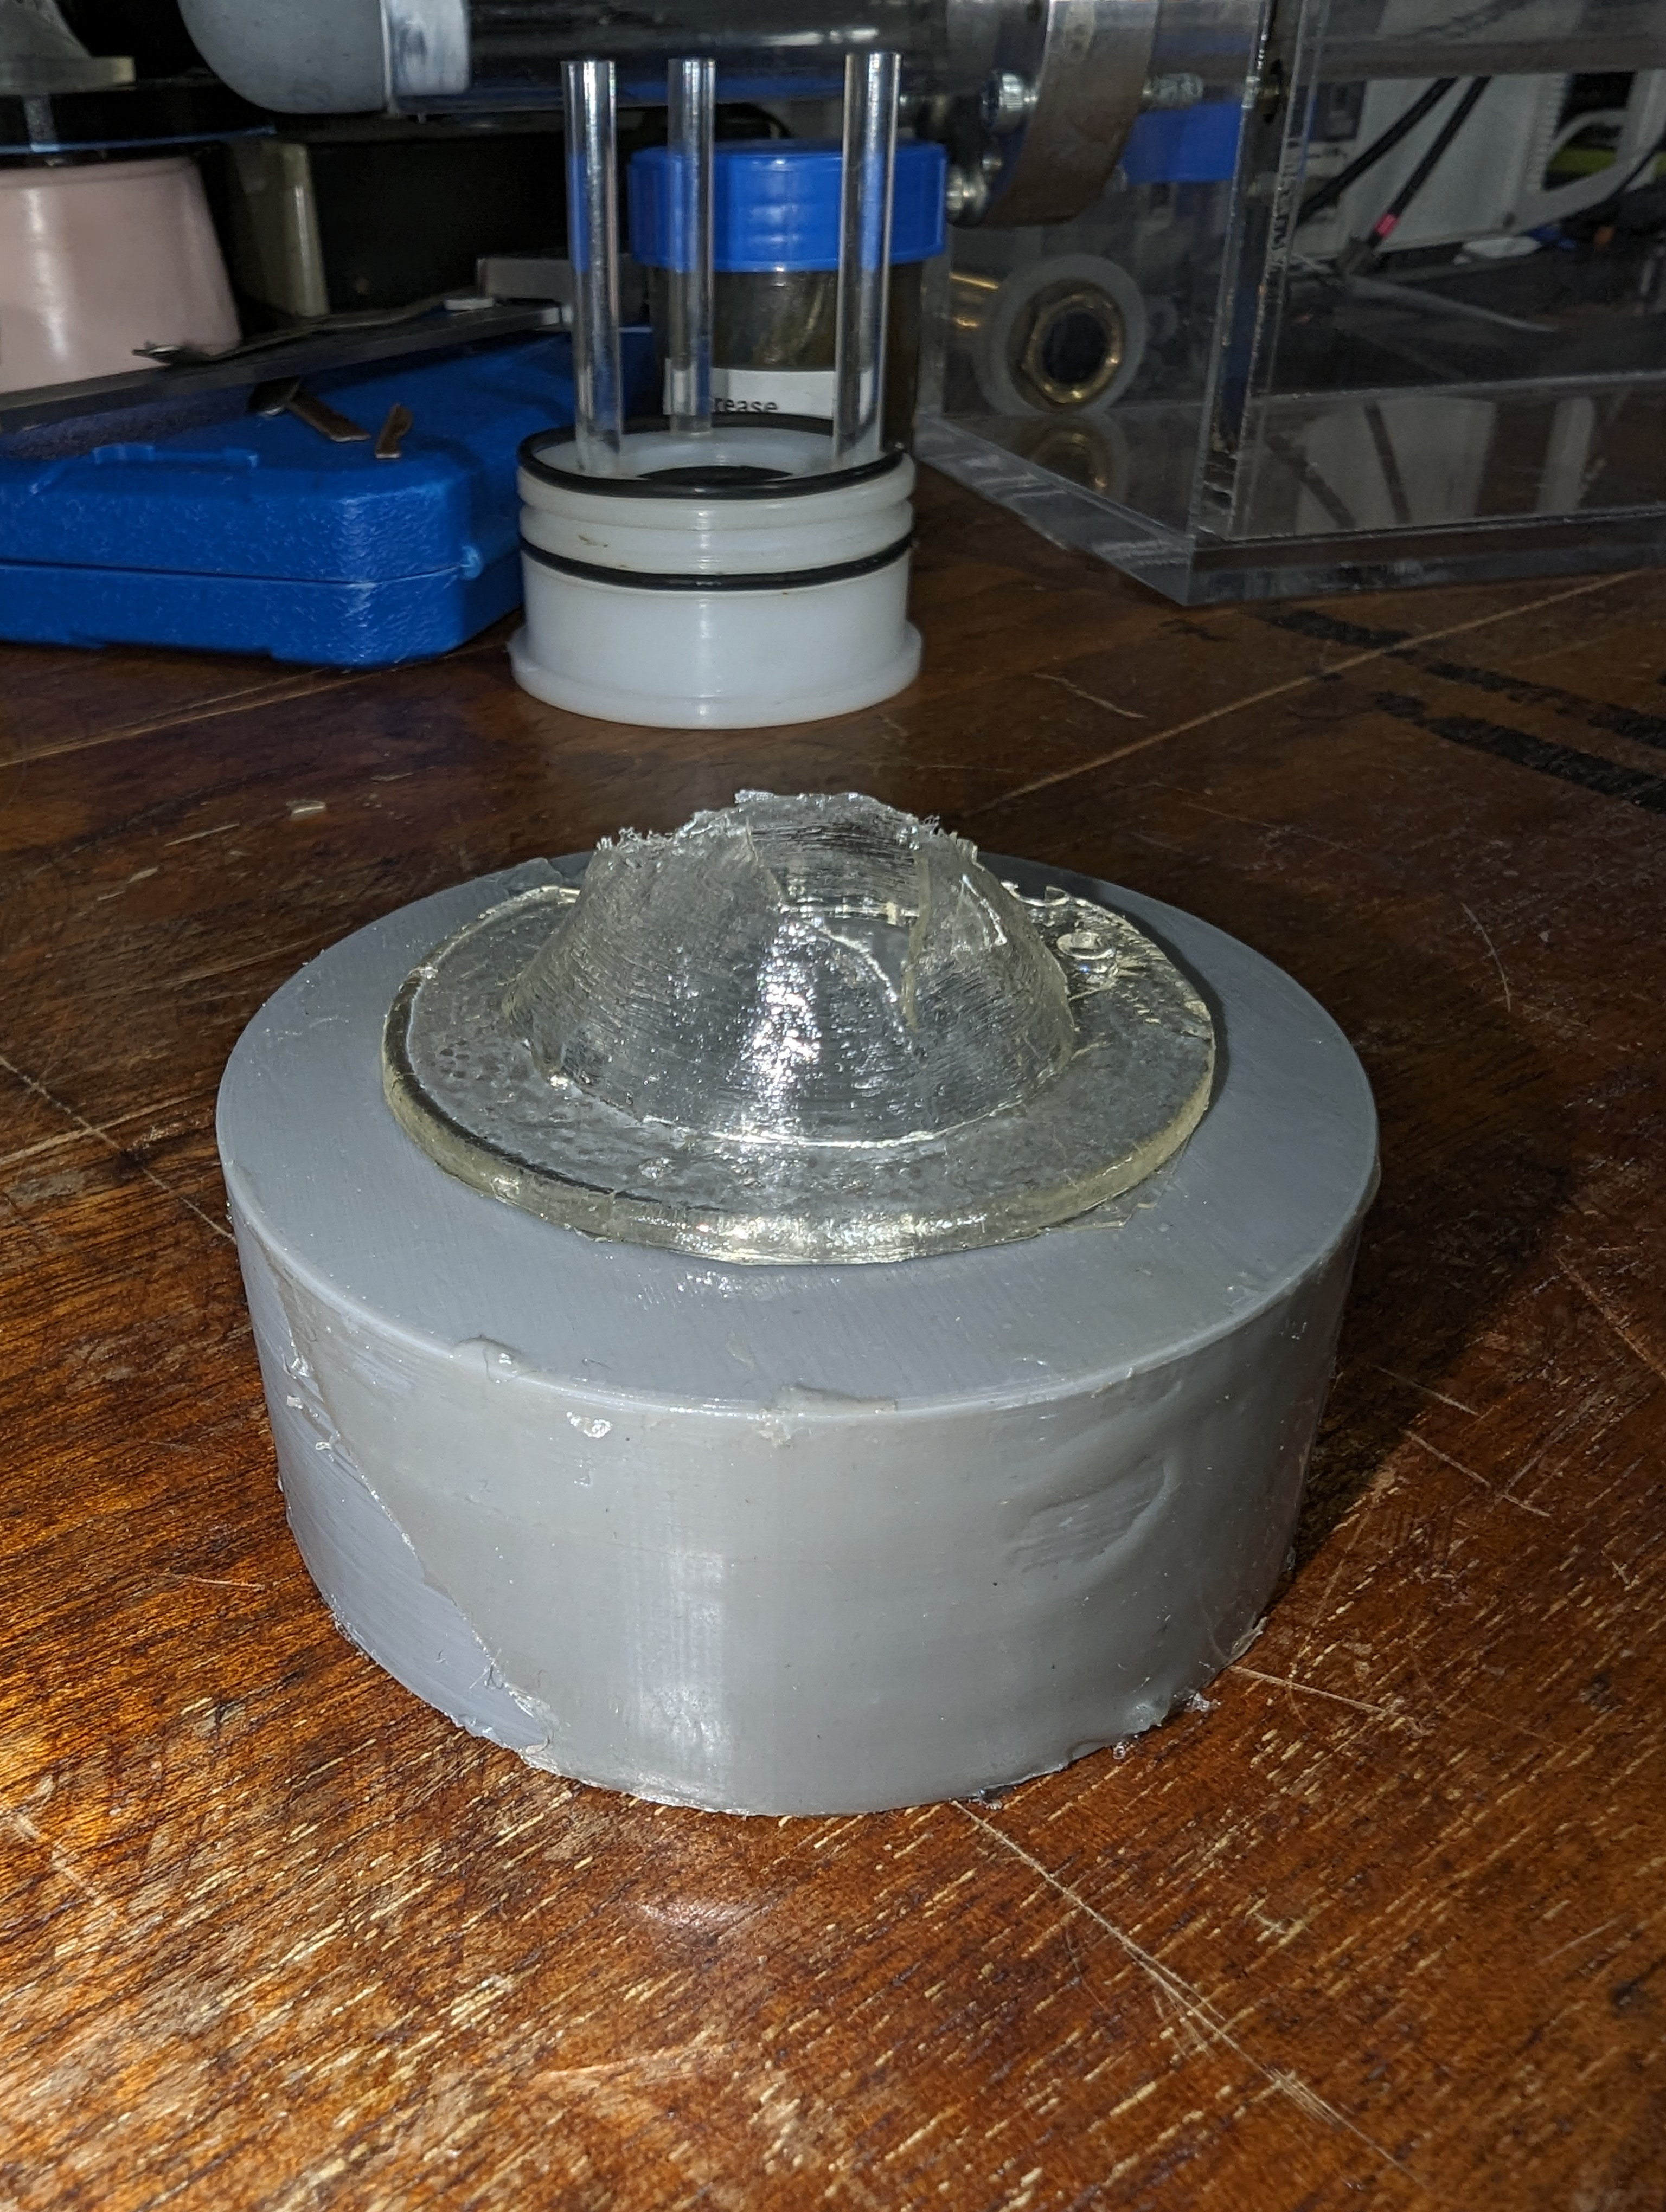
\includegraphics[width=0.75\textwidth]{figures/latercastnice.jpg}
    \caption{Final cast of anatomical valve}
    \label{fig:cast1}
\end{figure}

\newthought{Modelling}\\
Another area that caused an excess of time used was the post processing of the anatomical valve geometry, in becoming acquainted with STL modelling\sidenote{Software packages like blender use mainly sculpting tools that are used to modify the surface as opposed traditional CAD programs like SolidWorks where parts are built up from a tree of features} on the various programs trialed throughout the study the model was transferred across systems a lot to utilize the different tools each had, for example, how blender had great scuplting tools but lacked simple geometry analysis which was required for monitoring the surface as the thickness was homogenised.

While blender has capabilities to manipulate shaders to render this kind of information however due to it being an opensource program the process of developing a custom shader for this purpose was deemed too rescource intensive however if further work was conducted with many patient-specific models being developed it would be quite likely the most efficient option.

\newthought{Chordae Tendineae}\\
The tendineae attachment to the leaflets was another highly contested and thought out factor of the design. Balancing the rigidity that is added to the leaflets by some methods in attaching the nylon wire and the adhesion to the leaflet is very dificult, for the scope of this study it was found that B7000 adhesive worked well as the tendineae could be effectively attached with minimal disruption to the mechanics of the valve however this did add thickness to the leaflets which not only adds rigidity that hinders coaptation in experimental use but also brings many issues for potential computational simulations that could be conducted in tandem to a study of this nature.

Studies like \citeonly{karlExvivoInvitroDynamic2024} which had been examined in the later stages of the study use a method of embedding their chordae tendineae within the leaflets, containing a medical gauze matrix, so that the tendineae do not detach under tensile forces. An approach like this could prove very effective in application to this study as it would simplify the manufacturing process in that with a the tendineae can be attached to the gauze matrix prior to \gls{PU} casting ensuring accurate and replicable placement.

\newthought{Prototyping}\\
The prototyping conducted through the study for the mould parts, fixturing and experimental rig had many important  learnings. For each print the configuration of the printer was tailored to the purpose of the parts being produced, parts being made in early interations were set to faster infill and layer height settings to receive them faster whereas finalised ideas on slower higher resolution settings.

It was found these dense high definition settings had issues of their own to solve prints came out with an large amount of stringing which in certain cases was irrepairable. To circumnavigate this the researchers in the UCD print lab \todo{Word this properly} were consulted. Tailored settings in Prusa Slicer were programmed for the geometry where the resulting gcode would stop the nozzle from crossing the perimeter of the valve moulds, retraction settings would stop the printer from leaving blobs of plastic on the interior of the mould and z-axis seams were alligned to not interfere with the geometry either.

In earlier stages of the study a resin \gls{SLA} printer was used to manufacture an anatomic model that was to be used in the silicone mould method discussed in \cref{fig:silimould} which proved very effective however it was not feasible to develop further iterations regularly with this due to being part of a separate lab and the higher cost of the FormLabs proprietary resin. Two big benefits to \gls{SLA} printing are;

\begin{figure}[H]
    \centering
    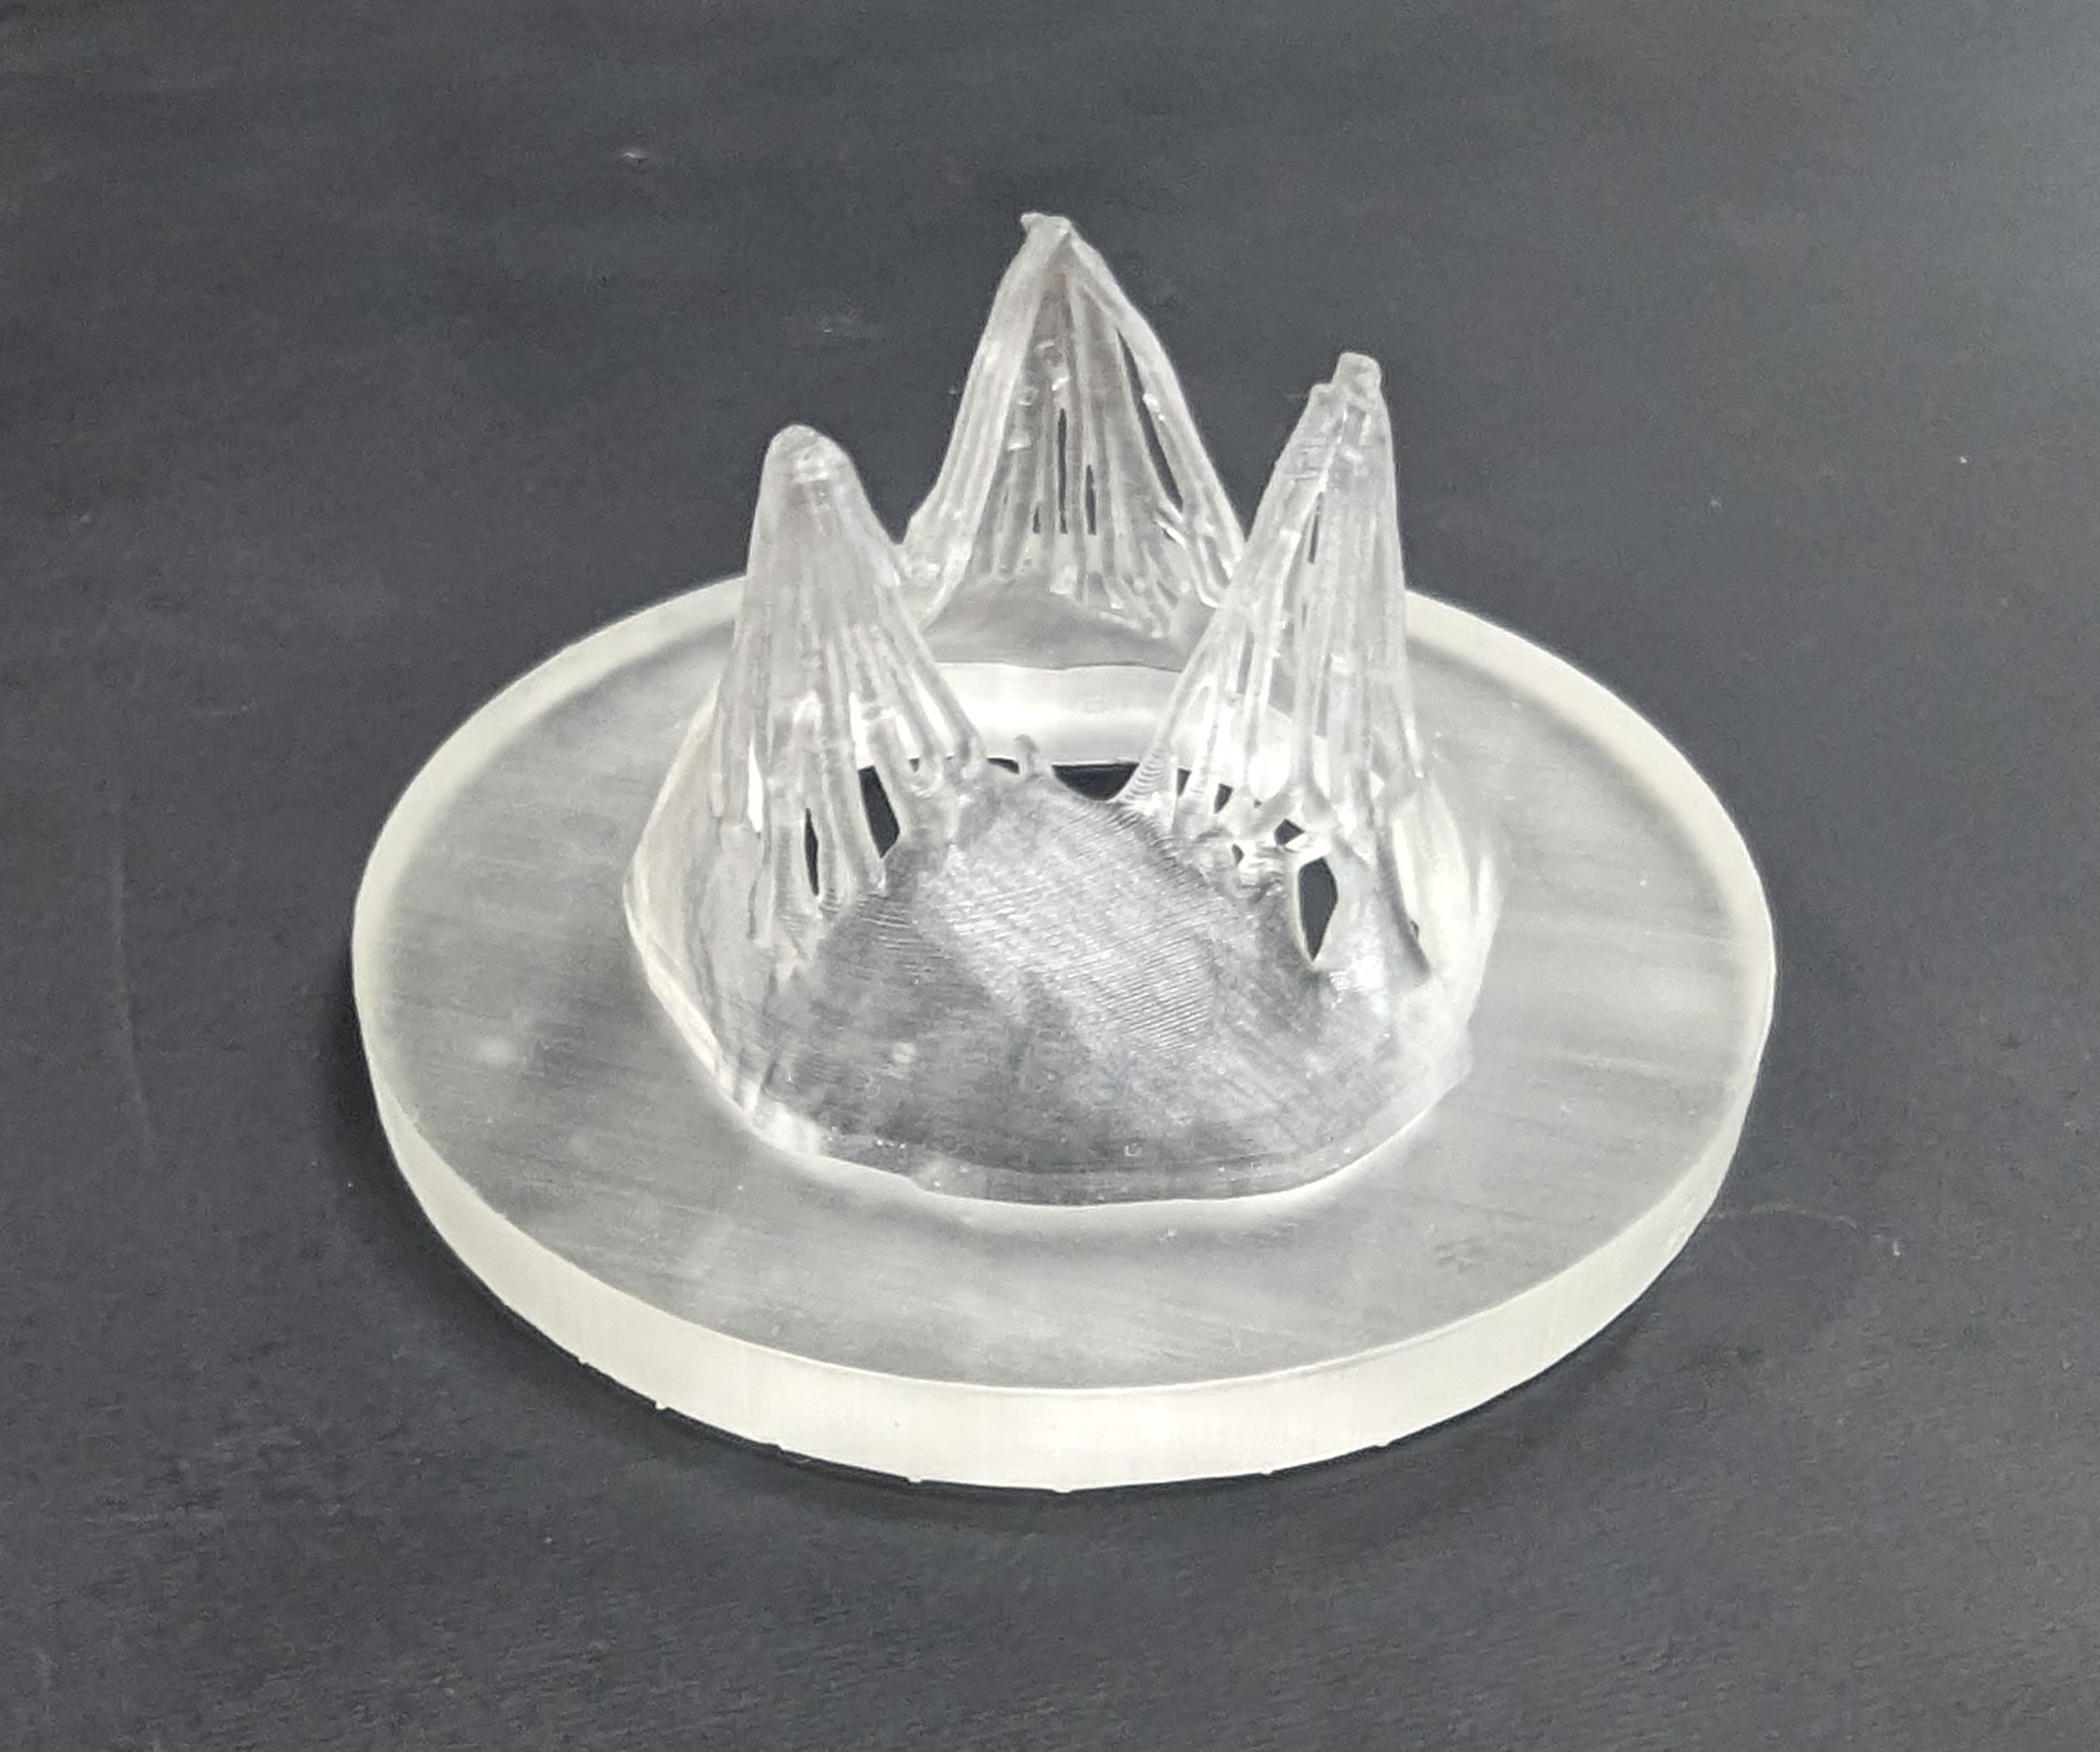
\includegraphics[width=0.75\textwidth]{figures/resinprintanat.jpg}
    \caption{Early revision \gls{SLA} print of anatomical valve}
    \label{fig:reso}
\end{figure}
\begin{itemize}
    \item The vastly increased tolerance of resin printing\\
          Prusa \gls{FDM}:0.3mm\\\todo{ref}
          FormLabs \gls{SLA}:0.01mm
    \item The reduced layer height that resin printing is capable of\\
          Prusa \gls{FDM}:0.05mm\\
          FormLabs \gls{SLA}:0.025mm
\end{itemize}
This has two bonuses for application in this study;
\begin{itemize}
    \item Minimizing layer height results in mould parts reduces surface affects
    \item Reducing adhesion of cast part to mould, this is minimized on \gls{PLA} parts with mould release and sanding however with casted parts on this degree of thickness there can still be an increased risk of breakage in the demoulding process.
\end{itemize}
Another option worth considering is machining from either steel or a performance plastic like delrin, this would be more expensive although it could be worth the cost for moulds that need to be used for a larger number of castings as well as increasing the precision over multiple casts since you the 3D printed parts can warp under the pressure of the clamping.

\section{Contextualizing Results}

% Discuss how your results relate to previous studies and theoretical frameworks. Are your findings consistent with other studies, or do they diverge?
% Analyze the significance of any discrepancies and explore possible reasons.

The results of this study have shown how development of imitative synthetic heart valves can be a valuable tool in cardiac simulators. The coaptation tests on the valve show great promise for technology of this nature, previously in simulational studies such as \todo{ref} dissected porcine valves, \todo{ref} used rigid valves and \todo{ref} non-anatomically representative valves which each have major limitations in their ability for a wider range of experiments.\\
Some such limitations of these valves which the work of this study has surpassed are;
\begin{itemize}
    \item The longevity of porcine for repeated experiments. While it can be stored in the likes of formalin the tissue degrades over time which leads to an irrepeatability in testing and eventual need for replacement.
    \item Semi-rigid valves can't be used in flow studies as they can't deform to coapt.
    \item Non-anatomical valves can coapt but don't represent true geometry which won't yield accurate results.
\end{itemize}

\mynewline
The coaptation test illustrated how the chordae tendineae can be used in a synthetic part to prevent prolapse and aid coaptation. The aligns well with how it had been done before such as in \citeonly{rabbahNovelLeftHeart2013} and \citeonly{karlExvivoInvitroDynamic2024} where native and synthetic tendineae were used respectively. Such works also show how this part of the model can be manipulated with motors to simulate the contraction of papillary muscles which while not applicable to the current design of the right heart simulator, could be developed for future iterations or simpler rig design like that of the tube-based coaptation test \cref{fig:Videos}

\subsection{Implications of the Findings}



\section{Reflecting}

% Acknowledge the limitations of your study and how they might affect the interpretation of your results.

The main shortcoming of this study is that the valve was not evaluated in the right heart simulator. This means that the flow field could not be measured with and without the CroiValve \gls{TTVR} device in place to characterize their efficacy on regurgitant valves.

\section{Future Research Directions}

% Based on your findings and the limitations identified, suggest areas for future investigation.

Pressure monitoring during test, 36\% glycerin for blood viscosity - rabbah

In vitro micro ct scanning

The next steps in this research would primarily be to fully integrate this valve into the right heart simulator. From there the rig would be enhanced so that fully representative simulations could be conducted where the flow field could be measured with and without \gls{TTVR} devices in place to characterize their efficacy on regurgitant valves. The main prospective device to integrate is the CroiValve DUO device which partially occludes the annulus of the valve reducing the regurgitant flow.

At the moment the CroiValve team don't have the means to conduct work of this nature so the data collected in this study could be used to inform the design inputs of later interations.